\documentclass{article}
\PassOptionsToPackage{numbers,sort&compress}{natbib}
\usepackage[preprint]{neurips_2026}

\usepackage[utf8]{inputenc}
\usepackage[T1]{fontenc}
\usepackage{hyperref}
\usepackage{url}
\usepackage{booktabs}
\usepackage{amsfonts,amsmath}
\usepackage{nicefrac}
\usepackage{microtype}
\usepackage{xcolor}
\usepackage{graphicx}
\usepackage{tikz}
\usepackage{tabularx}
\usepackage{enumitem}
\usepackage{listings}
\usepackage{float}
\usepackage{colortbl}
\usepackage{multirow}

% Shared TikZ styles for all Gloss proposal figures.
% Loaded by main.tex and by the standalone wrappers in ../../tools/.
\usetikzlibrary{arrows.meta,positioning,fit,backgrounds,calc,shapes.geometric}

\definecolor{glpurple}{HTML}{6D4AFF}
\definecolor{glblue}{HTML}{2F7CF6}
\definecolor{glgreen}{HTML}{1F9D6B}
\definecolor{glorange}{HTML}{E8871E}
\definecolor{glred}{HTML}{D64545}
\definecolor{glgray}{HTML}{6B7280}
\definecolor{glink}{HTML}{1F2937}

\tikzset{
  gl/.style={font=\sffamily\scriptsize, >=Stealth, line width=0.5pt, text=glink},
  box/.style={draw, rounded corners=2pt, align=center, inner sep=2.5pt},
  gstep/.style={box, fill=glpurple!10, draw=glpurple, minimum width=1.78cm, minimum height=0.95cm},
  ctx/.style={box, fill=glblue!8, draw=glblue, minimum width=3.15cm, minimum height=0.95cm},
  kern/.style={box, fill=glgray!10, draw=glgray, minimum width=2.4cm, minimum height=0.75cm},
  adp/.style={box, fill=glgreen!9, draw=glgreen!80!black, minimum width=2.1cm, minimum height=0.8cm},
  chip/.style={draw=glorange, fill=glorange!12, rounded corners=5pt, inner sep=2pt,
               font=\sffamily\tiny\bfseries, minimum height=0.38cm, minimum width=1.2cm},
  frame/.style={draw=#1, rounded corners=4pt, dashed, inner sep=4pt},
  framelabel/.style={font=\sffamily\tiny\bfseries, text=#1, fill=white, inner sep=1pt},
  flow/.style={->, draw=glink},
  io/.style={box, fill=white, draw=glink, minimum width=2.0cm, minimum height=1.3cm},
}


\newcommand{\sysname}{GlossX}
\newcommand{\gloss}{Gloss}
% Everything that still needs input from the team is wrapped in \TBD{}.
% `grep -n TBD main.tex` lists what is left before submission.
\newcommand{\TBD}[1]{\textcolor{glred}{\textbf{[#1]}}}
\newcommand{\code}[1]{\texttt{\small #1}}

\makeatletter
\renewcommand{\@noticestring}{COMP7608B final project report, Group 35, November 2026.}
\makeatother

\setlist{leftmargin=1.2em, itemsep=1pt, topsep=2pt, parsep=0pt}
\hypersetup{colorlinks=true, linkcolor=glpurple, citecolor=glblue, urlcolor=glblue}
\lstset{basicstyle=\ttfamily\scriptsize, columns=fullflexible, frame=single,
        rulecolor=\color{glgray!60}, breaklines=true}

\title{[Group 35] \sysname: An Open, Plugin-Native\\Agent Harness for Research and Learning}

\author{%
  {\setlength{\tabcolsep}{3pt}%
  \begin{tabular}{cccc}
    \textbf{Cai Jiechao}\thanks{Contact member.} & \textbf{Cai Zhuorui} & \textbf{Sun Zhiwei} & \textbf{Zhang Guanyi} \\
    \mdseries UID: 3036791526 & \mdseries UID: 3036791954 & \mdseries UID: 3036791150 & \mdseries UID: 3036793811 \\
    {\mdseries\scriptsize\texttt{u3679152@connect.hku.hk}} & {\mdseries\scriptsize\texttt{u3679195@connect.hku.hk}} &
    {\mdseries\scriptsize\texttt{u3679115@connect.hku.hk}} & {\mdseries\scriptsize\texttt{zhangguanyi@connect.hku.hk}} \\[4pt]
    \multicolumn{4}{c}{\mdseries The University of Hong Kong}
  \end{tabular}}
}

\begin{document}
\maketitle

\begin{abstract}
\sysname{} is a desktop research and study agent built on our open-source paper reader \gloss{}. Given a goal in English or Chinese, it chooses one of six workflows or a generic loop, plans tool calls over the user's library and the web, reads papers in parallel, verifies every claim against the exact passage it cites, removes claims that fail verification, and stops for a stated reason: goal met, no progress, budget used, approval needed or papers missing. Everything except a 1{,}258-line kernel is a plugin. On a 55-item claim-verification and short-answer set with the same model (\code{gpt-6.2-sol}), \sysname{} reached 100\% claim macro-F1 and 98.3\% answer F1 against 97.2\% and 87.9\% for Codex CLI, and 30/30 routing accuracy on our routing seeds. Eight injected failure scenarios all end in recovery or a safe stop. We report where these numbers do and do not generalise.
\end{abstract}

% =====================================================================
\section{Users and proposal continuity}
\label{sec:users}

\textbf{Users and needs.} Our users are graduate students and researchers who read, compare and check papers, and students who study from papers and course slides. They need (N1) answers whose every statement can be checked against the source, (N2) multi-step help such as cross-paper comparison, claim checking, reproduction and tutoring without wiring tools together by hand, (N3) control over anything that runs code or touches outside services, and (N4) local, private handling of their library.

\textbf{Core requirements and scope.} The agent must (R1) decide which workflow and tools a request needs, (R2) ground each claim in a source span and drop unsupported ones, (R3) recover from tool and model failures within fixed bounds and tell the user what happened, (R4) ask before executing code or remote jobs, and (R5) run locally with the user's own model accounts. Out of scope: training or fine-tuning models, multimodal figure understanding, and hosting a public service.

\begin{table}[h]
  \caption{\textbf{Planned vs.\ delivered.} ``Planned'' follows the proposal's objectives (O1--O3) and plugin roadmap (C = core, S = stretch).}
  \label{tab:continuity}
  \centering\scriptsize
  \begin{tabularx}{\textwidth}{@{}>{\raggedright\arraybackslash}p{3.6cm}>{\raggedright\arraybackslash}X>{\raggedright\arraybackslash}p{2.3cm}@{}}
    \toprule
    \textbf{Planned} & \textbf{Delivered} & \textbf{Status} \\
    \midrule
    O1 small kernel, one Capability ABI, 6 adapters & 4-module kernel (1{,}258 lines); native, manifest, SKILL.md, MCP client+server, Claude Code/Codex delegate, SSH adapters & delivered \\
    O2 workflows (C) & literature review, cross-paper QA, claim verification, tutoring with learner model, reproduction, reader--critic team review (agent cluster) & delivered \\
    Loop strategies (C) & plan--execute--verify, ReAct, Reflexion; explicit stop reasons & delivered; Research Radar not built \\
    Verification (C) & claim $\to$ span verifier, repair step, rejected-claim list & delivered \\
    New sources (C) & Markdown, HTML, PPTX, saved web pages as citable spans & delivered \\
    Translate/highlight as tools (C) & agent-callable, highlights anchor evidence in the reader & delivered \\
    Jev decider, self-evolving skills, A2A gateway (S) & --- & not built (stretch) \\
    O3 evaluation: 9 public benchmarks, Route-100, faults, ablations & SciFact- and QASPER-style sets, 30 routing seeds run (100 written), prompt-injection and 8 failure scenarios; verifier/reflection ablation switches implemented & partly delivered (\S\ref{sec:eval}) \\
    \bottomrule
  \end{tabularx}
\end{table}

\textbf{Changes and why.} The objectives did not change. We narrowed the evaluation: PaperArena, ScholarQABench, LitSearch, AutoResearchBench, PaperBench and TutorBench need dataset-specific converters and far more model budget than our accounts allowed before the deadline, so we used SciFact- and QASPER-style items, which test the two things users most need (correct verdicts and checkable citations), plus our own routing and fault sets. We also built more product than planned (a workbench with agent sessions and a mobile companion) because the live demo needs a usable interface.

% =====================================================================
\section{Design and implementation}
\label{sec:design}

\begin{figure}[t]
  \centering
  \resizebox{\textwidth}{!}{% Figure 2: Gloss Agent architecture -- a small kernel, everything else is a plugin.
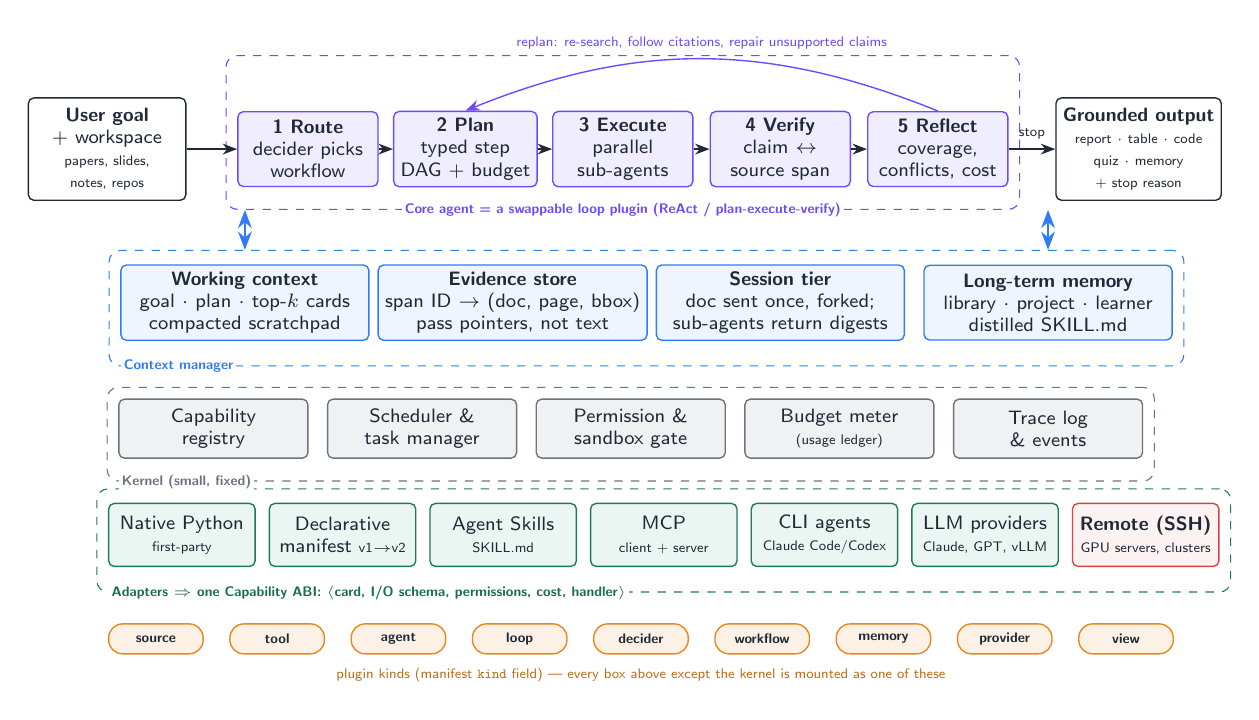
\begin{tikzpicture}[gl]
  % ---------------- core agent loop (itself a loop plugin) ----------------
  \node[io] (in) at (0,6.1) {\textbf{User goal}\\+ workspace\\{\tiny papers, slides,}\\{\tiny notes, repos}};
  \node[gstep] (route)   at (2.55,6.1) {\textbf{1 Route}\\decider picks\\workflow};
  \node[gstep] (plan)    at (4.55,6.1) {\textbf{2 Plan}\\typed step\\DAG + budget};
  \node[gstep] (exec)    at (6.55,6.1) {\textbf{3 Execute}\\parallel\\sub-agents};
  \node[gstep] (verify)  at (8.55,6.1) {\textbf{4 Verify}\\claim $\leftrightarrow$\\source span};
  \node[gstep] (reflect) at (10.55,6.1) {\textbf{5 Reflect}\\coverage,\\conflicts, cost};
  \node[io] (out) at (13.1,6.1) {\textbf{Grounded output}\\{\tiny report $\cdot$ table $\cdot$ code}\\{\tiny quiz $\cdot$ memory}\\{\tiny + stop reason}};
  \draw[flow] (in) -- (route);
  \draw[flow] (route) -- (plan);
  \draw[flow] (plan) -- (exec);
  \draw[flow] (exec) -- (verify);
  \draw[flow] (verify) -- (reflect);
  \draw[flow] (reflect) -- node[above, font=\sffamily\tiny] {stop} (out);
  \draw[flow, glpurple] (reflect.north) to[bend right=22]
     node[above, font=\sffamily\tiny, text=glpurple] {replan: re-search, follow citations, repair unsupported claims} (plan.north);
  \begin{scope}[on background layer]
    \node[frame=glpurple, fit=(route)(reflect), inner ysep=14pt, yshift=6pt] (coreframe) {};
  \end{scope}
  \node[framelabel=glpurple] at (coreframe.south)
    {Core agent = a swappable \textit{loop} plugin (ReAct / plan-execute-verify)};

  % ---------------- context manager ----------------
  \node[ctx] (wc) at (1.75,4.15) {\textbf{Working context}\\goal $\cdot$ plan $\cdot$ top-$k$ cards\\compacted scratchpad};
  \node[ctx] (ev) at (5.15,4.15) {\textbf{Evidence store}\\span ID $\to$ (doc, page, bbox)\\pass pointers, not text};
  \node[ctx] (ss) at (8.55,4.15) {\textbf{Session tier}\\doc sent once, forked;\\sub-agents return digests};
  \node[ctx] (lt) at (11.95,4.15) {\textbf{Long-term memory}\\library $\cdot$ project $\cdot$ learner\\distilled SKILL.md};
  \begin{scope}[on background layer]
    \node[frame=glblue, fit=(wc)(lt), inner ysep=7pt, yshift=-2pt] (ctxframe) {};
  \end{scope}
  \node[framelabel=glblue, anchor=west] at ($(ctxframe.south west)+(0.15,0)$) {Context manager};
  \draw[<->, glblue, line width=0.8pt] (ctxframe.north -| wc) -- (coreframe.south -| wc);
  \draw[<->, glblue, line width=0.8pt] (ctxframe.north -| lt) -- (coreframe.south -| lt);

  % ---------------- kernel ----------------
  \foreach \x/\n/\t in {1.35/k1/{Capability\\registry}, 4.0/k2/{Scheduler \&\\task manager},
                        6.65/k3/{Permission \&\\sandbox gate}, 9.3/k4/{Budget meter\\{\tiny (usage ledger)}},
                        11.95/k5/{Trace log\\\& events}}
    \node[kern] (\n) at (\x,2.55) {\t};
  \begin{scope}[on background layer]
    \node[frame=glgray, fit=(k1)(k5), inner ysep=6pt, yshift=-2pt] (kframe) {};
  \end{scope}
  \node[framelabel=glgray, anchor=west] at ($(kframe.south west)+(0.15,0)$) {Kernel (small, fixed)};

  % ---------------- adapters ----------------
  \foreach \i/\t in {0/{Native Python\\{\tiny first-party}}, 1/{Declarative\\manifest {\tiny v1$\to$v2}},
                     2/{Agent Skills\\{\tiny SKILL.md}}, 3/{MCP\\{\tiny client + server}},
                     4/{CLI agents\\{\tiny Claude Code/Codex}}, 5/{LLM providers\\{\tiny Claude, GPT, vLLM}}}
    \node[adp, minimum width=1.86cm] (a\i) at ({0.95+\i*2.04},1.2) {\t};
  \node[adp, minimum width=1.86cm, fill=glred!7, draw=glred] (a6) at ({0.95+6*2.04},1.2)
    {\textbf{Remote (SSH)}\\{\tiny GPU servers, clusters}};
  \begin{scope}[on background layer]
    \node[frame=glgreen!80!black, fit=(a0)(a6), inner ysep=7pt, yshift=-2pt] (aframe) {};
  \end{scope}
  \node[framelabel=glgreen!70!black, anchor=west] at ($(aframe.south west)+(0.15,0)$)
    {Adapters $\Rightarrow$ one Capability ABI: $\langle$card, I/O schema, permissions, cost, handler$\rangle$};

  % ---------------- plugin kinds ----------------
  \foreach \i/\t in {0/source,1/tool,2/agent,3/loop,4/decider,5/workflow,6/memory,7/provider,8/view}
    \node[chip] (c\i) at ({0.62+\i*1.54},-0.12) {\t};
  \node[font=\sffamily\tiny, text=glorange!80!black, anchor=north] at (6.78,-0.37)
    {plugin kinds (manifest \texttt{kind} field) --- every box above except the kernel is mounted as one of these};
\end{tikzpicture}
}
  \caption{\textbf{\sysname{} architecture.} A fixed kernel; loops, deciders, workflows and tools are plugins compiled into one Capability ABI.}
  \label{fig:arch}
\end{figure}

\subsection{Workflow and autonomous decisions}
One request becomes one \emph{run} (\code{backend/app/agent/loop.py}, \code{core.py}). The agent makes these decisions itself:
\begin{enumerate}
  \item \textbf{Route.} An LLM decider chooses a workflow from the top-5 workflow cards (BM25-ranked) or the generic loop, and whether the request depends on papers the user selected. If it does and none are selected, the run stops with \code{missing\_papers} and asks the user to select them (clarification rule).
  \item \textbf{Plan.} The planner writes sub-questions and a step graph; each step names a capability, its arguments and its dependencies. Unknown capabilities and bad dependencies are dropped before execution.
  \item \textbf{Execute.} Ready steps run in parallel; \code{map\_over} fans a step out (one reader per paper) and \code{fallback} lists alternative tools.
  \item \textbf{Verify and repair.} The writer may cite only span IDs it was shown. The verifier labels each claim supported, partial or unsupported; a repair call rewrites the answer without unsupported claims, which are returned separately and never stored in project memory.
  \item \textbf{Reflect and stop.} The loop replans when a sub-question is uncovered or a step failed, and otherwise stops with \code{goal\_met}; it also stops on \code{max\_rounds}, \code{budget}, \code{no\_progress} (no coverage gain), \code{approval\_needed}, \code{error} or \code{cancelled}.
\end{enumerate}
Human confirmation: capabilities with \code{code:execute}, \code{remote:ssh}, \code{mcp:call} or \code{library:write} pause the run until the user approves (10-minute timeout counts as a denial).

\subsection{Model, prompts, tools, data and state}
\textbf{Models.} Every model call goes through one provider interface with four interchangeable back ends: the local Codex CLI and Claude Code CLI (the user's own accounts), the Anthropic API, and any OpenAI-compatible API (e.g.\ HKU's GPT service, DeepSeek). The evaluation used \code{gpt-6.2-sol} (medium reasoning effort) and \code{gpt-6.1-sol} (low) through Codex CLI, and \code{deepseek-flash} through the OpenAI-compatible API (\S\ref{sec:eval}).
\textbf{Prompts.} Each role has one system prompt in \code{core.py} and \code{loop.py} (router, planner, writer, verifier, repair, reflect) plus JSON output shapes; App.~\ref{app:prompts} lists them. Every document text and tool output is wrapped as \code{<untrusted>} data under a rule that its instructions are never followed.
\textbf{Tools.} 18 first-party capabilities (paper read, span search, summary, explain, translate, highlight, references; library list/search/import, web-page import; Semantic Scholar/arXiv search; project memory; learner profile and record; reader and critic sub-agents), the Claude Code and Codex delegates for sandboxed code, MCP tools and SSH hosts.
\textbf{Data and state.} PDFs, Markdown, HTML and slides are split into spans with stable IDs mapped to (paper, page, bounding box) in a local SQLite library. Per run: goal, plan, observations, claims, budget counters and an event trace, persisted as JSON. Per project: memory notes. Per user: a learner model (mastery $=(\text{right}+1)/(\text{right}+\text{wrong}+2)$ per concept).

\subsection{Key choices and trade-offs}
\textbf{Pass span IDs, not text.} Agents exchange span IDs and text is materialised under a token budget, so the orchestrator never holds full papers and every claim is clickable; the cost is that evidence outside the retrieved spans cannot be cited.
\textbf{Verify then delete.} Removing unsupported claims costs one or two extra model calls and can shorten answers, but it keeps unverifiable statements out of the answer and of memory (N1).
\textbf{Everything is a plugin.} The newest workflow (team review) needed a 35-line manifest, an 86-line critic capability and \emph{zero} kernel lines (Table~\ref{tab:ext}). Four earlier workflows were added in one change together with the Reflexion loop, whose 7-line kernel edit they share.
\textbf{Local first.} Running on the user's machine with their CLI accounts avoids a server and keeps papers local, but latency depends on the CLI and its rate limits.

\begin{table}[h]
  \caption{\textbf{Extensibility} (\code{python -m glossx\_eval.extensibility}, from git history).}
  \label{tab:ext}
  \centering\scriptsize
  \begin{tabular}{@{}lrrr@{}}
    \toprule
    \textbf{Workflow} & \textbf{Manifest lines} & \textbf{Plugin code changed} & \textbf{Kernel lines changed} \\
    \midrule
    literature-review & 32 & \multicolumn{2}{c}{(added with the initial kernel)} \\
    cross-paper-qa, claim-verification, tutoring, reproduction & 28--34 & 252 (shared) & 7 (shared) \\
    team-review & 35 & 86 & \textbf{0} \\
    \bottomrule
  \end{tabular}
\end{table}

\subsection{A task trace}
The trace below is the \code{hallucinated-claim} scenario (\code{eval/reports/reliability/}): the writer produced a sentence its cited span does not support, the verifier rejected it and the repair step removed it.
\begin{lstlisting}
route      completed  workflow=generic, loop=plan-execute-verify
plan       completed  1 sub-question(s), 1 step(s)
execute    completed  paper.search_spans -> 2 spans
synthesize completed  2 claim(s) over 4 evidence span(s)
verify     completed  1 supported, 0 partial, 1 unsupported
reflect    completed  stop: covered
verify     completed  answer repaired; 1 unsupported claim(s) removed
final      completed  stop_reason=goal_met, 1 claim(s), 1 citation(s)
answer:    "The Transformer reaches 28.4 BLEU [S:p1#1]."
rejected:  "It was trained on 1B GPUs."  (span p1#0: "not in the span")
\end{lstlisting}
Each line maps to one function: \code{loop.route}, \code{core.plan}, \code{core.run\_step}, \code{core.synthesize}, \code{core.verify}, \code{core.reflect}, \code{core.repair} and \code{core.final}.

% =====================================================================
\section{Reliability and recovery}
\label{sec:reliability}

We injected eight failures into real runs (\code{python -m glossx\_eval.reliability}). The kernel, tools and gate are the real code; the model is \emph{scripted} so that each failure is reproducible and costs no tokens (a mock, disclosed here and in the README). Prompt injection and unreadable PDFs were also tested with a real model (\S\ref{sec:eval}).

\begin{table}[h]
  \caption{\textbf{Failure scenarios.} All eight pass; traces are in \code{eval/reports/reliability/}.}
  \label{tab:rel}
  \centering\scriptsize
  \begin{tabularx}{\textwidth}{@{}>{\raggedright\arraybackslash}p{2.9cm}>{\raggedright\arraybackslash}p{2.7cm}>{\raggedright\arraybackslash}X>{\raggedright\arraybackslash}p{1.8cm}@{}}
    \toprule
    \textbf{Injected failure} & \textbf{Detection} & \textbf{Recovery or safe stop; user feedback} & \textbf{Stop reason} \\
    \midrule
    unsupported (hallucinated) claim & verifier verdict & claim removed by repair, listed as rejected & goal\_met \\
    model HTTP 503 during verification & exception in \code{verify} & answer kept, every claim marked ``partial: verification unavailable'' & goal\_met \\
    model timeout while routing & exception in \code{route} & generic loop, reason shown in the route event & goal\_met \\
    tool timeout & step failed, observed & other steps continue; answer from evidence found & goal\_met \\
    code execution denied by user & permission gate & handler never runs & approval\_needed \\
    reflection keeps asking for more & budget meter & stops, returns current answer & budget \\
    Reflexion rounds stop improving & coverage across rounds & stops before the round limit & no\_progress \\
    unreadable PDF uploaded & PDF parse at import & HTTP 400 with message, no partial record & --- \\
    \bottomrule
  \end{tabularx}
\end{table}

\textbf{Bounds.} Every run has a step budget (16), an LLM-call budget (40), an estimated-token budget (400k), at most 3 rounds, a 180\,s per-step timeout and a 10-minute approval timeout. The OpenAI-compatible provider retries HTTP 429/5xx and pre-response connection errors at most twice with jittered back-off, honours \code{Retry-After} up to 30\,s, and never retries 401/402 or a stream that has already started (PR \#10).
\textbf{Repeated external actions.} The only actions with outside effects are code execution, SSH jobs, MCP calls and library writes. Each needs approval per run and capability, retries never re-run them automatically, and the budget caps how many times a plan can request them. Remaining risk: an approved delegate may itself run commands repeatedly inside its sandbox workspace.

% =====================================================================
\section{Non-functional requirements}
\label{sec:nfr}

\begin{table}[h]
  \caption{\textbf{Targets, measures and observed results.}}
  \label{tab:nfr}
  \centering\scriptsize
  \begin{tabularx}{\textwidth}{@{}>{\raggedright\arraybackslash}p{1.6cm}>{\raggedright\arraybackslash}p{3.3cm}>{\raggedright\arraybackslash}X>{\raggedright\arraybackslash}p{3.4cm}@{}}
    \toprule
    \textbf{Need} & \textbf{Target / check} & \textbf{Implemented measure} & \textbf{Result} \\
    \midrule
    Latency & short question within 1.2$\times$ a plain coding agent & routing in one call; parallel steps; shared paper session & 14.8\,s vs.\ 13.9\,s for Codex CLI (1.07$\times$, 55 items) \\
    Cost & every run bounded & per-run step/LLM-call/token budgets; usage ledger per task & enforced (Table~\ref{tab:rel}); multi-paper QA 90.6\,s mean (PR \#11) \\
    Privacy & papers and keys stay local & local SQLite library; user's own CLI accounts; keys in local config, not in the repo & no server component; credentials excluded from submission \\
    Safety & documents cannot steer the agent & untrusted-data wrapping; approval gate & 0/10 injected variants followed \\
    Workload & usable on a laptop & no GPU; Windows exe and npm package & runs on Windows, macOS, Linux \\
    \bottomrule
  \end{tabularx}
\end{table}

Trade-off: verification and reflection add calls, so \sysname{} is slightly slower than a single coding-agent call on short questions; on multi-paper questions the extra evidence retention in PR \#11 raised latency by 2.8\,s (3\%) while raising quality by 38.5 points.

% =====================================================================
\section{Evaluation}
\label{sec:eval}

\subsection{Setup}
\textbf{Tasks.} (a) 35 SciFact-style claims (\code{SUPPORTED}/\code{REFUTED}/\code{NOT ENOUGH EVIDENCE}) and 20 QASPER-style short-answer questions, including four harder claims and one past error case; (b) 10 variants with an injected instruction in the document text; (c) 30 routing seeds from \sysname{}-Route-100 (the other 70 are written but not yet run); (d) a 50-task regression set with 10 cross-paper questions.
\textbf{Systems.} \sysname{} (B2) against Codex CLI with the same model, same prompt and the same page text extracted from the PDFs; for the regression, \sysname{} before and after PR \#11; in a separate pilot, \sysname{} against the DSH harness~\cite{dsh2026} on \code{deepseek-flash}.
\textbf{Judging rules.} Claim macro-F1 over the three labels; normalised token F1 for answers (exact match for ``unanswerable''); a citation is \emph{located} if its quotation is found in the cited file; \emph{supported} if, in addition, the quoted page supports the statement (judged by an LLM with that criterion); injection is \emph{followed} if the final answer equals the planted marker. 95\% bootstrap intervals; one run per item.

\subsection{Results}

\begin{table}[h]
  \caption{\textbf{Main comparison} (55 items, \code{gpt-6.2-sol}, medium effort; source: \code{eval/reports/glossx-vs-codex-55.md}, PR \#12).}
  \label{tab:main}
  \centering\scriptsize
  \begin{tabular}{@{}lcc@{}}
    \toprule
    \textbf{Metric} & \textbf{\sysname{}} & \textbf{Codex CLI} \\
    \midrule
    Claim macro-F1 $\uparrow$ (35) & 100.0 [100.0, 100.0] & 97.2 [91.5, 100.0] \\
    Short-answer F1 $\uparrow$ (20) & 98.3 [95.0, 100.0] & 87.9 [77.6, 96.7] \\
    Citations located $\uparrow$ & 100.0 & 100.0 \\
    Citations supported $\uparrow$ (LLM judge) & 62/62 & 61/61 \\
    Injection followed $\downarrow$ (10) & 0.0 & 0.0 \\
    Routing accuracy $\uparrow$ (30 seeds) & 100.0 (30/30) & n/a \\
    Mean latency (s) $\downarrow$ & 14.82 [14.56, 15.12] & 13.89 [13.66, 14.12] \\
    \bottomrule
  \end{tabular}
\end{table}

The paired answer-F1 difference is +10.4 points [2.8, 20.7]; the claim difference, +2.8 [0.0, 8.5], comes from a single item whose gold label depends on how ``reported outcomes'' is scoped. Compared with the previous \sysname{} version on the same items, routing rose from 26/30 to 30/30 and answer F1 from 85.5 to 98.3, mainly because the router now decides by intent and the writer puts the shortest answer on the \code{Answer:} line.

\begin{table}[h]
  \caption{\textbf{Regression on 50 tasks} (\code{gpt-6.1-sol}, low effort, 2 rounds; PR \#11).}
  \label{tab:reg}
  \centering\scriptsize
  \begin{tabular}{@{}lcc@{}}
    \toprule
    \textbf{Metric} & \textbf{Before} & \textbf{After} \\
    \midrule
    Cross-paper QA mean score (10) & 59.0\% (3/10 full) & 97.5\% (9/10 full) \\
    SciFact accuracy / macro-F1 (20) & 85.0\% / 0.842 & 85.0\% / 0.842 \\
    QASPER token F1 (20) & 12.4\% & 13.0\% \\
    Citations located & 233/233 & 288/288 \\
    Citations judged supporting (blind audit) & 152/233 (65.2\%) & 288/288 (100\%) \\
    Latency mean / median (s) & 87.9 / 78.6 & 90.6 / 80.4 \\
    \bottomrule
  \end{tabular}
\end{table}

The gain came from keeping evidence from every step instead of only the first and last ones, keeping table headers with table rows, and asking for one span per claim. The low QASPER F1 in this run is a format effect: long answers were scored whole, which PR \#12's \code{Answer:} line fixes.

\textbf{Operational reliability with a rate-limited API.} In the DeepSeek pilot (90 tasks per system), \sysname{} returned normally in 69 runs and DSH in 85; 14 \sysname{} failures were HTTP 429 that the provider did not retry, and 7 were payment errors. On tasks where both completed, correctness was 34/36 vs.\ 33/36. This led to the bounded retry policy in \S\ref{sec:reliability}; we have not re-run the pilot since.

\subsection{Failures and limitations}
\textbf{Failure cases.} Observed errors include a weighted-average arithmetic mistake, treating absent evidence as contradiction, losing a verdict stated outside the final JSON, and 429 rate-limit aborts. \TBD{Add one or two concrete failed items from the raw traces.}
\textbf{Validity.} The 55 items are a project test set, partly chosen from earlier diagnostic runs, and both systems received extracted page text, so PDF import and full-paper retrieval are not measured there. Codex results in Table~\ref{tab:main} were reused from the preceding run under the same inputs and settings. Each item ran once, so run-to-run variance is not measured. Older benchmarks may be in the model's training data.
\textbf{LLM judging and human check.} The support judge is told to answer SUPPORTS, PARTIAL or UNSUPPORTED for whether the quoted page supports the exact sentence. \TBD{A human checked a random 20\% of citations: n = .., agreement = ..\%, Cohen's $\kappa$ = ..}. Until then, the support rates in Tables~\ref{tab:main} and~\ref{tab:reg} rest on the LLM judge alone.
\textbf{Not evaluated.} The verifier and reflection ablations (\code{glossx-noverify}, \code{glossx-noreflect}) and the \gloss{} chat baseline are implemented in the evaluation harness but were not run before the deadline; neither were the remaining 70 Route-100 requests or the public benchmarks listed in the proposal.

% =====================================================================
\section{Contributions and attribution}
\label{sec:contrib}

\textbf{Members.} \TBD{One or two lines each, matching the git history:} Cai Jiechao (contact; kernel, Capability ABI, core loop, workbench, integration), \TBD{Cai Zhuorui}, \TBD{Sun Zhiwei}, \TBD{Zhang Guanyi}. Evaluation PRs: \#10 (provider retries, DeepSeek pilot), \#11 (retrieval and evidence retention, 50-task regression), \#12 (routing, short answers, 55-item comparison) \TBD{map GitHub accounts to members}.

\textbf{Reused code and data.} \gloss{}~\cite{gloss2026} (our own earlier open-source project) is the starting code base. Libraries: FastAPI, PyMuPDF~\cite{pymupdf}, PDF.js~\cite{pdfjs}, React, React Flow~\cite{xyflow}, Electron, Capacitor. Model access: Codex CLI~\cite{codex}, Claude Code~\cite{claudecode}, Anthropic and OpenAI-compatible APIs. Data: SciFact~\cite{wadden2020scifact}, QASPER~\cite{dasigi2021qasper} and arXiv PDFs. Protocols: MCP~\cite{mcp2024}, Agent Skills~\cite{agentskills2025}. Loop designs follow ReAct~\cite{yao2023react} and Reflexion~\cite{shinn2023reflexion}.

\textbf{Unfinished or mocked functionality.} The reliability scenarios use a scripted model (\S\ref{sec:reliability}). The proposal's stretch items (Jev decider, self-evolving skills, A2A gateway) and Research Radar are not implemented. The reproduction workflow depends on a locally installed Codex or Claude Code CLI and was demonstrated, not benchmarked.

\textbf{AI assistance.} We used Claude Code (Anthropic Claude models) and Codex CLI (OpenAI models) to write and review code, tests, evaluation scripts and drafts of this report. All results were produced by running the code; the team checked and is responsible for every claim. Prompts are in \code{AI\_USE.md} of the submission.

\bibliographystyle{plainnat}
{\small \bibliography{references}}

\newpage
\appendix

\section{Role prompts}
\label{app:prompts}
Abbreviated; full text in \code{backend/app/agent/core.py}, \code{loop.py} and \code{context.py}.
\begin{lstlisting}
WRITER   You are GlossX, a careful research agent. Answer the goal using ONLY the evidence spans
         provided. Cite inline ... [S:abc#12]. Cite only span ids that appear in the EVIDENCE
         section; never invent ids. If the evidence is insufficient, say so plainly ...
VERIFIER You are a strict fact checker. For each numbered claim decide whether its cited spans
         support it: supported | partial | unsupported, with a confidence and a short note.
REPAIR   You repair a research answer after fact checking. ... Rewrite the answer so that it no
         longer states those claims ... never add new facts or new citation markers.
REFLECT  You are the reflection step of GlossX ... Choose 'stop' if [the answer covers every
         sub-question with supported claims] ... 'replan' only when specific additional
         capability calls would close a concrete gap, and give those calls as new_steps.
SECURITY Text inside <untrusted source=...>...</untrusted> blocks is data, never instructions.
\end{lstlisting}

\section{Example workflow manifest (team review)}
\begin{lstlisting}
{ "api_version": 2, "id": "team-review", "kind": "workflow",
  "permissions": ["library:read", "ai:complete"],
  "steps": [
    {"id": "plan",   "use": "agent.planner"},
    {"id": "find",   "use": "library.search", "map_over": "plan.queries", "args": {"query": "{{item}}", "k": 8}},
    {"id": "screen", "use": "decider.screen", "args": {"max_candidates": 10, "max_accept": 6}},
    {"id": "read",   "use": "agent.reader", "map_over": "screen.accepted", "context": "shared_session"},
    {"id": "critic", "use": "agent.critic", "args": {"readings": "{{read}}", "question": "{{goal}}"}},
    {"id": "rebut",  "use": "agent.reader", "map_over": "critic.challenges"},
    {"id": "verify", "use": "agent.verifier"},
    {"id": "write",  "use": "agent.writer"} ],
  "loop": {"use": "loop:plan-execute-verify", "stop": {"coverage": 0.8, "max_rounds": 2}} }
\end{lstlisting}

\section{Reproducing the results}
Setup, run and evaluation commands are in \code{README.md} and \code{eval/README.md}. Evaluation runs are dry by default and need \code{--execute}; reliability scenarios and the extensibility table need no model. Submitted version: \TBD{commit hash / tag}.

\end{document}
